\documentclass[11pt,border=5pt]{standalone}
\usepackage{fontspec}
\setmainfont{cmunrm.otf}[BoldFont=cmunbx.otf,ItalicFont=cmunti.otf,BoldItalicFont=cmunbi.otf]
\usepackage{amsmath}
\usepackage{unicode-math}
\setmathfont{NewCMMath-Regular.otf}
\usepackage{tikz}
\usetikzlibrary{arrows.meta,patterns,angles,quotes}
\begin{document}
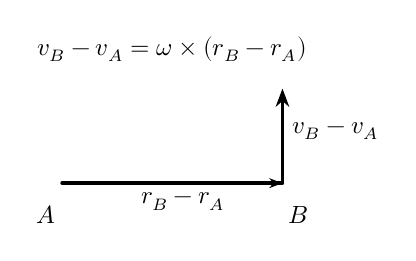
\begin{tikzpicture}[>=Stealth,font=\small,line cap=round,line join=round]
\draw[very thick] (-1.4,0) -- (1.4,0);
\node at (-1.6,-0.4) {$A$};
\node at (1.6,-0.4) {$B$};
\draw[->,thick] (1.4,0) -- (1.4,1.2) node[pos=0.55,right] {$v_B-v_A$};
\draw[->,thin,dashed] (-1.4,0) -- (1.4,0) node[pos=0.55,below] {$r_B-r_A$};
\node at (0,1.7) {$v_B-v_A=\omega\times(r_B-r_A)$};

\end{tikzpicture}
\end{document}
